\documentclass[11pt]{article}
\usepackage[margin=1in]{geometry}
\usepackage{graphicx,booktabs,amsmath,amssymb,hyperref,xcolor}
\usepackage{caption}
\title{LeJudge: a cost module you program in English\\\large Natural-language constraints for JEPA world-model planning with a decision model in the loop}
\author{Abdel \and (agent-built draft)}
\date{\today}
\begin{document}
\maketitle

\begin{abstract}
LeWorldModel (LeWM) plans by minimising one number: the latent distance between an imagined final state and a goal image. That cost cannot say ``but not through there'' or ``keep it upright''. LeJudge adds a natural-language cost module: linear probes turn each imagined LeWM latent into a handful of words, Jev (TypeSafe's System One decision model) answers one typed yes/no question per imagined step per constraint, and code folds the calibrated probabilities into the CEM cost. No LLM runs in the planning loop and no text is generated. On PushT with a library of twelve constraints across three families, at the pre-registered penalty weight $\lambda=1$ the episode violation rate was \VAL{jev_violation_all} for LeJudge against \VAL{lewm_violation_all} for unconstrained LeWM, with success \VAL{jev_success_all} vs \VAL{lewm_success_all}; the oracle-on-probes upper bound, which shares the code path with a perfect judge, reached \VAL{oracle_violation_all}, so at this weight the bottleneck is the cost mechanics and the conflict between goal and constraint, not the judge. The $\lambda$ sweep and the satisfiable-episode stratification (Section~3) quantify what the penalty can and cannot change. In the judge-only study Jev's accuracy on five held-out paraphrases per constraint was \VAL{jev_para_acc} against \VAL{jev_canon_acc} on the canonical text, while a keyword checker dropped from \VAL{kw_canon_acc} to \VAL{kw_para_acc}. Every response is cached; all figures regenerate offline.
\end{abstract}

\section{Introduction}
JEPA-style world models draw a configurable cost module on the architecture diagram; LeJudge is a small, measured instance of one that a non-expert can configure in plain English. The method is \emph{imagine} $\rightarrow$ \emph{describe} $\rightarrow$ \emph{judge} $\rightarrow$ \emph{decide}: LeWM imagines latent futures; probes describe each imagined latent as words from a closed vocabulary; Jev judges typed questions about those words; the planner decides.

\section{Method}
\paragraph{Probes and vocabulary.} Linear heads map the 192-d post-projector LeWM latent to agent position, block position, block angle ($\sin,\cos$) and contact. A deterministic vocabulary buckets these into a $3\times3$ grid cell, an edge flag, six angle bins, a contact flag and a speed word. No number ever reaches the judge. On encoded expert frames the linear probe reaches $R^2 = \VAL{probe_r2_block}$ (block position), $\VAL{probe_r2_angle}$ (angle); bucket accuracy \VAL{probe_bucket_block} (block cell), \VAL{probe_bucket_angle} (angle bin), \VAL{probe_bucket_edge} (edge). Over five imagined steps block-cell accuracy falls to \VAL{probe_bucket_block_h5} (Fig.~\ref{fig:err}).
\paragraph{Constraint library.} Twelve PushT constraints in three families (\texttt{never}, \texttt{always}, \texttt{soft}), each with an oracle checker on ground-truth state, five paraphrases and two near-miss negatives (library \texttt{pusht-lib@1}, SHA-256 \texttt{\VAL{library_sha}}).
\paragraph{Judge.} State = \{\texttt{constraints}: owner text, \texttt{candidates}: code-generated facts\}; one Noul per (constraint, step) for the hard families (\texttt{never}, \texttt{always}) and one Score per (candidate, constraint) for \texttt{soft}. Aggregation ($\max$, $1-\min$, $1-\mathbb{E}[\mathrm{level}]/4$) and a confidence gate are Python.
\paragraph{Cost.} $\mathrm{cost} = \mathrm{std}(A) + \lambda \sum_c w_c\,\mathrm{penalty}_c$ over \emph{all} $S=300$ candidates, with $A = \lVert \hat z_H - z_g \rVert^2$ standardised per iteration; $\lambda=0$ is bit-identical to LeWM. Because a hard-family question depends only on one step's words and its index, the population's $S \times H$ steps collapse to unique (step, facts) keys that are judged once and memoised across iterations, replans and episodes (persistent table shared by every run); soft constraints are judged on the $K=16$ lowest-cost candidates, the rest receiving the shortlist's mean penalty as a prior. CEM iterations $0, 5, \dots, 25$ and the last are judged (\VAL{cem_iters} iterations in total). An earlier design that judged only a $K=16$ shortlist on the last three iterations could not change plans even with a perfect (oracle) judge; the change was logged before any Jev result on the study sets (\texttt{docs/DECISIONS.md}).

\section{Experiments}
\paragraph{Setup.} PushT (\texttt{stable-worldmodel} \texttt{swm/PushT-v1}), LeWM checkpoint \texttt{quentinll/lewm-pusht} (revision \texttt{\VAL{ckpt_rev}}), the authors' protocol (goal 25 env steps ahead, budget 50, CEM $300\times30$, horizon 5 blocks of 5 steps, history 3). Reproduction gate: unconstrained success \VAL{m0_success} on \VAL{m0_n} episodes. Conditions share start states, goals and sampler seeds.
\paragraph{Judge-only study (Table~\ref{tab:judge}, Fig.~\ref{fig:para}, Fig.~\ref{fig:rel}).} \VAL{judge_n_items} items (executed windows described with ground-truth words and with probe words; imagined CEM candidates described with probe words, labelled by oracle-on-probes) $\times$ 12 constraints $\times$ 8 texts.
\paragraph{Planning study (Table~\ref{tab:plan}, Fig.~\ref{fig:sv}).} Conditions \{LeWM, oracle-on-probes, keyword, Jev\VAL{llm_cond_note}\} $\times$ sets \{spatial = [centre\_avoid], spatial+temporal = [centre\_avoid, no\_contact\_first3], implicit = [gentle, approach\_below]\}, \VAL{plan_episodes} episodes per cell and seed, seeds \VAL{plan_seeds}. Bootstrap 95\% CIs (10,000 resamples); paired Wilcoxon vs LeWM with Holm correction across sets. The RFC's \texttt{edges} sets were replaced before the study because the expert start/goal windows almost never bring the block to a side wall (DECISIONS). Post hoc (exploratory) we stratify episodes by whether the constraint set is \emph{satisfiable} from the start and goal states: in the spatial set \VAL{spatial_unsat_frac} of episodes have the goal block in the centre cell, so success and compliance are mutually exclusive by construction. On satisfiable episodes, LeWM violates \VAL{lewm_violation_sat} and LeJudge \VAL{jev_violation_sat} (oracle-on-probes \VAL{oracle_violation_sat}); on the satisfiable spatial episodes every condition produced identical plans, i.e. no imagined candidate entered the centre cell and the executed violations are imagination-versus-execution error of the world model. Paired Wilcoxon tests of every condition against LeWM are not significant after Holm correction (Table~\ref{tab:plan}, \texttt{table2b\_paired\_tests}). Jev's confidence gate held \VAL{jev_abstention_spatial} of judged candidates on the spatial set.

\paragraph{Study 2: relevance-filtered starts (Table~\ref{tab:plan2}).} Pre-registered after Study 1 (\texttt{docs/PREREG.md}): start/goal windows are kept only when the set is satisfiable from both end states and the expert's own trajectory between them violates it, so task and constraint are in tension by construction (dataset-only filter, identical for every condition; same conditions, sets, seeds and budgets). Episode violation rates (LeWM / oracle-on-probes / keyword / Jev): spatial \VAL{lewm_violation_filt_spatial} / \VAL{oracle_violation_filt_spatial} / \VAL{keyword_violation_filt_spatial} / \VAL{jev_violation_filt_spatial}; spatial+temporal \VAL{lewm_violation_filt_spatial_temporal} / \VAL{oracle_violation_filt_spatial_temporal} / \VAL{keyword_violation_filt_spatial_temporal} / \VAL{jev_violation_filt_spatial_temporal}; implicit \VAL{lewm_violation_filt_implicit} / \VAL{oracle_violation_filt_implicit} / \VAL{keyword_violation_filt_implicit} / \VAL{jev_violation_filt_implicit}. Success for Jev vs LeWM: \VAL{jev_success_filt_all} vs \VAL{lewm_success_filt_all}. With a perfect judge the chosen plan is imagined to violate in only about a fifth of the filtered spatial episodes while execution violates in three quarters: the residual is the world model's open-loop drift over the 25-step receding horizon (replanning every block drops unconstrained success to 30\%, and executing the best sampled candidate instead of the elite mean changes little), not the judge. Where compliant paths are reachable (spatial+temporal, implicit) the oracle and even the keyword checker reduce violations by 8--14 points (Holm-corrected paired Wilcoxon significant for three cells) with no loss of success, whereas Jev moves by 3--4 points: its pre-registered confidence gate ($\tau = 0.5$ on the fraction of per-step probabilities in $[0.3, 0.7]$) zeroed the penalty for 21--62\% of candidates. The gate, not Jev's accuracy, is the binding constraint; re-tuning it after seeing these numbers would have been a post-hoc change, so we report it as the next experiment.

\paragraph{Study 3: the confidence gate (Table~\ref{tab:gate}).} Pre-registered after Study 2. Jev on the two responsive sets with the same filtered episodes and $\tau \in \{0.75, 1.0\}$ ($\tau = 1$ disables the gate). Violation (spatial+temporal / implicit): $\tau=0.5$ \VAL{jev_violation_filt_spatial_temporal} / \VAL{jev_violation_filt_implicit}; $\tau=0.75$ \VAL{jev_violation_gate075_spatial_temporal} / \VAL{jev_violation_gate075_implicit}; $\tau=1.0$ \VAL{jev_violation_gate10_spatial_temporal} / \VAL{jev_violation_gate10_implicit} (oracle-on-probes \VAL{oracle_violation_filt_spatial_temporal} / \VAL{oracle_violation_filt_implicit}). Success with the gate off: \VAL{jev_success_gate10_all}.

\begin{table}[h]\centering\caption{Study 3: Jev with the confidence gate at $\tau \in \{0.5, 0.75, 1.0\}$ next to the Study 2 baselines on the same episodes.}\label{tab:gate}
\begin{tabular}{llllllllll}
\toprule
condition & constraint\_set & n & success & success\_lo & success\_hi & violation & violation\_lo & violation\_hi & abstention\_rate \\
\midrule
jev:tau0.5 & implicit & 90 & 0.733 & 0.644 & 0.822 & 0.733 & 0.633 & 0.822 & 0.213 \\
jev:tau0.75 & implicit & 90 & 0.656 & 0.556 & 0.756 & 0.767 & 0.678 & 0.856 & 0.098 \\
jev:tau1.0 & implicit & 90 & 0.722 & 0.633 & 0.811 & 0.689 & 0.589 & 0.778 & 0.000 \\
keyword & implicit & 90 & 0.711 & 0.611 & 0.800 & 0.656 & 0.556 & 0.756 & 0.000 \\
lewm & implicit & 90 & 0.711 & 0.622 & 0.800 & 0.767 & 0.678 & 0.856 & 0.000 \\
oracle & implicit & 90 & 0.667 & 0.567 & 0.756 & 0.689 & 0.589 & 0.789 & 0.000 \\
jev:tau0.5 & spatial+temporal & 90 & 0.722 & 0.633 & 0.811 & 0.567 & 0.467 & 0.667 & 0.226 \\
jev:tau0.75 & spatial+temporal & 90 & 0.678 & 0.578 & 0.778 & 0.567 & 0.467 & 0.667 & 0.088 \\
jev:tau1.0 & spatial+temporal & 90 & 0.633 & 0.533 & 0.733 & 0.556 & 0.456 & 0.656 & 0.000 \\
keyword & spatial+temporal & 90 & 0.678 & 0.578 & 0.767 & 0.467 & 0.367 & 0.567 & 0.000 \\
lewm & spatial+temporal & 90 & 0.644 & 0.544 & 0.744 & 0.611 & 0.511 & 0.711 & 0.000 \\
oracle & spatial+temporal & 90 & 0.644 & 0.544 & 0.744 & 0.511 & 0.411 & 0.611 & 0.000 \\
\bottomrule
\end{tabular}
\end{table}

\begin{table}[h]\centering\caption{Study 2 (relevance-filtered starts): success and episode violation with 95\% bootstrap CIs.}\label{tab:plan2}
\begin{tabular}{lllllllllll}
\toprule
condition & constraint\_set & n & success & success\_lo & success\_hi & violation & violation\_lo & violation\_hi & plan\_p50\_s & judge\_calls\_per\_episode \\
\midrule
jev & implicit & 90 & 0.733 & 0.644 & 0.822 & 0.733 & 0.633 & 0.822 & 4.740 & 12.644 \\
keyword & implicit & 90 & 0.711 & 0.611 & 0.800 & 0.656 & 0.556 & 0.756 & 1.634 & 0.000 \\
lewm & implicit & 90 & 0.711 & 0.622 & 0.800 & 0.767 & 0.678 & 0.856 & 1.603 & 0.000 \\
oracle & implicit & 90 & 0.667 & 0.567 & 0.756 & 0.689 & 0.589 & 0.789 & 2.207 & 0.000 \\
jev & spatial & 90 & 0.933 & 0.878 & 0.978 & 0.878 & 0.811 & 0.944 & 2.060 & 1.311 \\
keyword & spatial & 90 & 0.922 & 0.867 & 0.978 & 0.922 & 0.867 & 0.967 & 3.024 & 0.000 \\
lewm & spatial & 90 & 0.922 & 0.867 & 0.967 & 0.867 & 0.789 & 0.933 & 1.316 & 0.000 \\
oracle & spatial & 90 & 0.922 & 0.867 & 0.978 & 0.922 & 0.867 & 0.967 & 1.616 & 0.000 \\
jev & spatial+temporal & 90 & 0.722 & 0.633 & 0.811 & 0.567 & 0.467 & 0.667 & 2.593 & 2.400 \\
keyword & spatial+temporal & 90 & 0.678 & 0.578 & 0.767 & 0.467 & 0.367 & 0.567 & 1.974 & 0.000 \\
lewm & spatial+temporal & 90 & 0.644 & 0.544 & 0.744 & 0.611 & 0.511 & 0.711 & 1.561 & 0.000 \\
oracle & spatial+temporal & 90 & 0.644 & 0.544 & 0.744 & 0.511 & 0.411 & 0.611 & 2.072 & 0.000 \\
\bottomrule
\end{tabular}
\end{table}

\begin{table}[h]\centering\caption{Judge-only metrics (canonical text; probe-word items). Accuracy at 0.5, AUROC, ECE (10 equal-mass bins), paraphrase accuracy, near-miss negative false-positive rate, wall-clock per 1,000 judgments.}\label{tab:judge}
\begin{tabular}{llllllllll}
\toprule
judge & source & description & n\_items & canonical\_accuracy & canonical\_auroc & canonical\_ece & paraphrase\_accuracy & negative\_fpr & latency\_ms\_per\_1000 \\
\midrule
jev & executed & gt-words & 64 & 0.883 & 0.955 & 0.113 & 0.858 & 0.535 & 2458.217 \\
jev & executed & probe-words & 64 & 0.862 & 0.939 & 0.083 & 0.853 & 0.529 & 2458.217 \\
jev & imagined & probe-words & 128 & 0.881 & 0.937 & 0.107 & 0.871 & 0.383 & 2561.187 \\
keyword & executed & gt-words & 64 & 0.898 & 0.918 & 0.075 & 0.642 & 0.025 & 0.000 \\
keyword & executed & probe-words & 64 & 0.884 & 0.901 & 0.086 & 0.642 & 0.024 & 0.000 \\
keyword & imagined & probe-words & 128 & 0.894 & 0.895 & 0.086 & 0.738 & 0.020 & 0.000 \\
llm & executed & gt-words & 8 & 0.615 & 0.611 & 0.332 & 0.000 & nan & 565954.823 \\
llm & executed & probe-words & 8 & 0.594 & 0.588 & 0.356 & 0.000 & nan & 565954.823 \\
oracle & executed & gt-words & 64 & 0.971 & 1.000 & 0.013 & 0.971 & nan & 0.000 \\
oracle & executed & probe-words & 64 & 0.971 & 1.000 & 0.013 & 0.971 & nan & 0.000 \\
oracle & imagined & probe-words & 128 & 0.986 & 1.000 & 0.003 & 0.986 & nan & 0.000 \\
\bottomrule
\end{tabular}
\end{table}

\begin{table}[h]\centering\caption{Planning study: success and episode violation rate with 95\% bootstrap CIs; planning time per replan; judge calls per episode.}\label{tab:plan}
\begin{tabular}{lllllllllll}
\toprule
condition & constraint\_set & n & success & success\_lo & success\_hi & violation & violation\_lo & violation\_hi & plan\_p50\_s & judge\_calls\_per\_episode \\
\midrule
jev & implicit & 90 & 0.844 & 0.767 & 0.911 & 0.589 & 0.489 & 0.689 & 4.315 & 12.633 \\
keyword & implicit & 90 & 0.822 & 0.744 & 0.900 & 0.556 & 0.456 & 0.656 & 1.478 & 0.000 \\
lewm & implicit & 90 & 0.844 & 0.767 & 0.911 & 0.567 & 0.467 & 0.667 & 3.793 & 0.000 \\
oracle & implicit & 90 & 0.822 & 0.733 & 0.900 & 0.522 & 0.422 & 0.622 & 1.659 & 0.000 \\
jev & spatial & 90 & 0.844 & 0.767 & 0.911 & 0.556 & 0.456 & 0.656 & 2.327 & 3.122 \\
keyword & spatial & 90 & 0.811 & 0.722 & 0.889 & 0.556 & 0.456 & 0.656 & 1.412 & 0.000 \\
lewm & spatial & 90 & 0.844 & 0.767 & 0.911 & 0.567 & 0.467 & 0.667 & 1.000 & 0.000 \\
oracle & spatial & 90 & 0.811 & 0.722 & 0.889 & 0.556 & 0.456 & 0.656 & 1.531 & 0.000 \\
jev & spatial+temporal & 90 & 0.844 & 0.767 & 0.911 & 0.844 & 0.767 & 0.911 & 2.248 & 3.122 \\
keyword & spatial+temporal & 90 & 0.844 & 0.767 & 0.911 & 0.811 & 0.722 & 0.889 & 1.482 & 0.000 \\
lewm & spatial+temporal & 90 & 0.844 & 0.767 & 0.911 & 0.856 & 0.778 & 0.922 & 1.218 & 0.000 \\
oracle & spatial+temporal & 90 & 0.833 & 0.756 & 0.900 & 0.833 & 0.756 & 0.911 & 1.773 & 0.000 \\
\bottomrule
\end{tabular}
\end{table}

\begin{figure}[h]\centering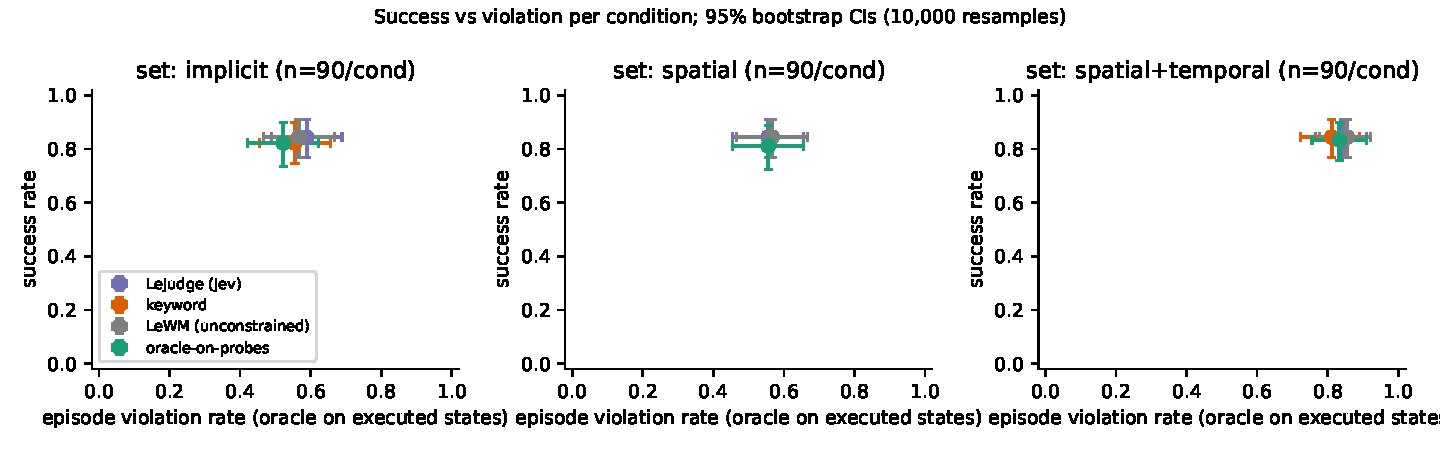
\includegraphics[width=\linewidth]{figures/fig2_success_vs_violation.pdf}\caption{Success vs violation per condition and constraint set.}\label{fig:sv}\end{figure}
\begin{figure}[h]\centering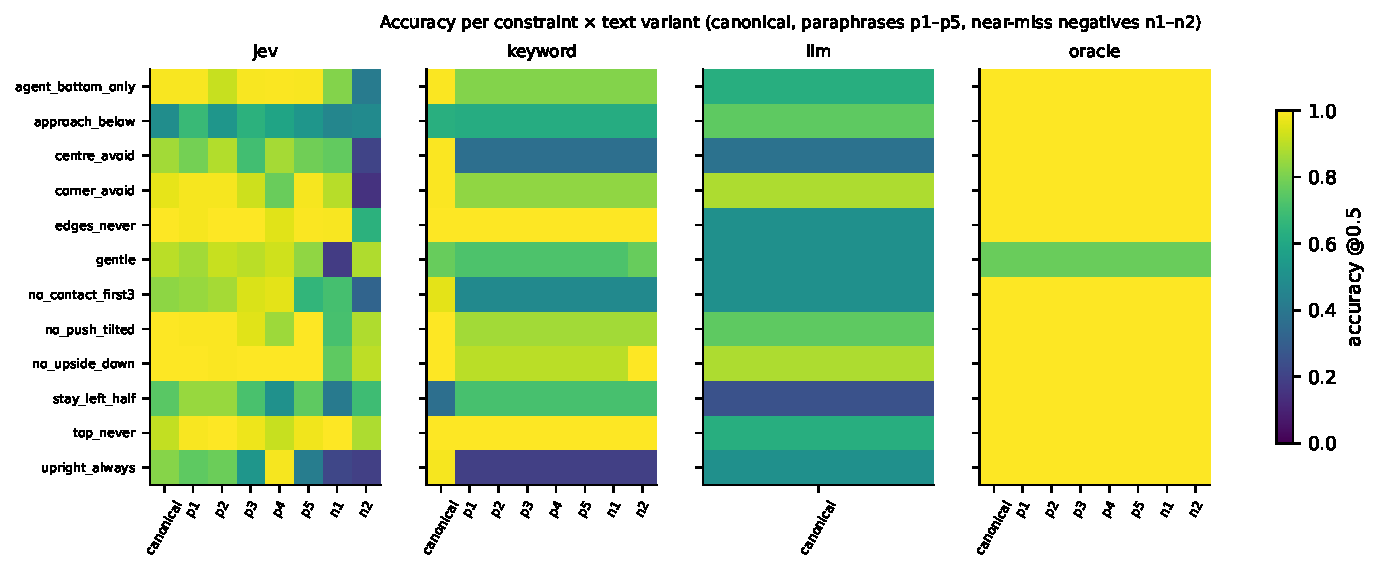
\includegraphics[width=0.9\linewidth]{figures/fig4_paraphrase_heatmap.pdf}\caption{Accuracy per constraint and text variant.}\label{fig:para}\end{figure}
\begin{figure}[h]\centering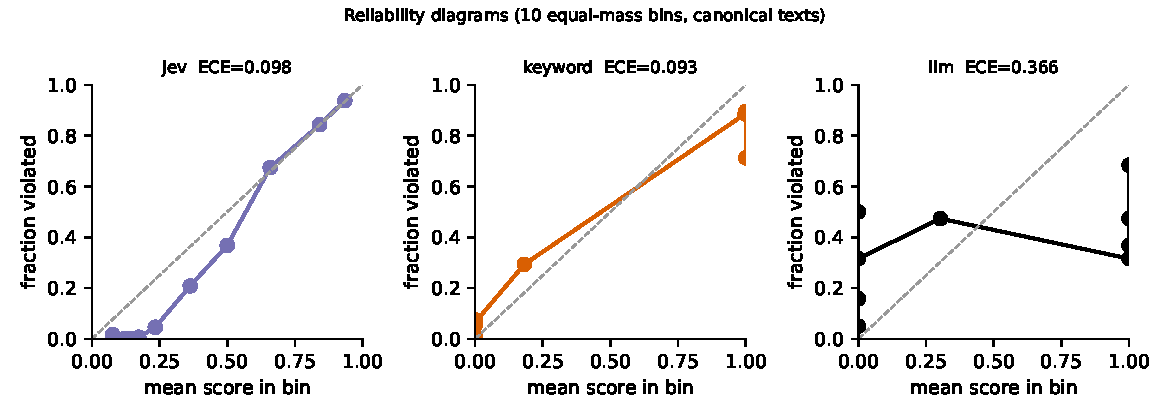
\includegraphics[width=0.8\linewidth]{figures/fig6_reliability.pdf}\caption{Reliability diagrams.}\label{fig:rel}\end{figure}
\begin{figure}[h]\centering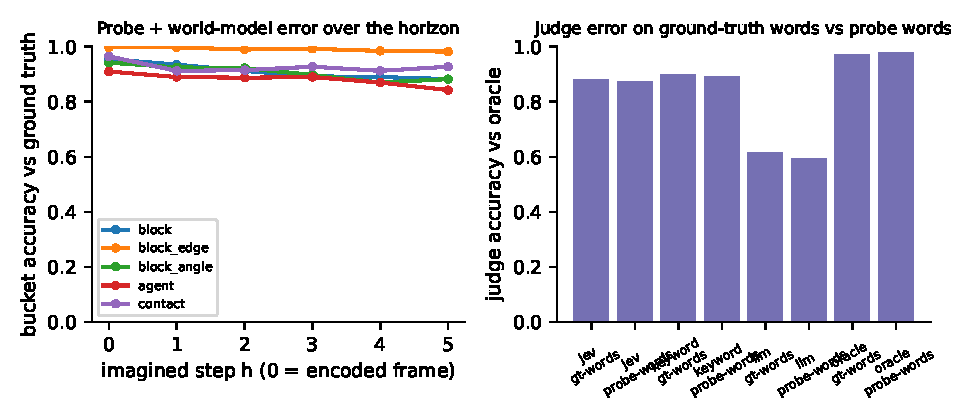
\includegraphics[width=0.9\linewidth]{figures/fig7_error_decomposition.pdf}\caption{Error decomposition: probe and world-model error over the horizon; judge error on ground-truth words vs probe words.}\label{fig:err}\end{figure}

\section{Limitations}
PushT only; twelve constraints; the world model's imagination error dominates beyond a few steps; Jev is a closed model (responses are cached and pinned to \texttt{\VAL{jev_model}}); the small-LLM baseline is \VAL{llm_note}.

\section{Reproducibility}
\texttt{make paper} regenerates every figure and number from \texttt{artifacts/results/*.parquet} with \texttt{LEJUDGE\_MODE=offline}; the Jev cache holds \VAL{cache_n} responses. Constraint texts and facts never share a state field.
\end{document}
